\section{The Large Hadron Collider}
In March 1984, the European Organization for Nuclear Research CERN) and the European Committee for Future Accelerators (ECFA) 
held a workshop in Lausanne entitled "Large Hadron Collider in the LEP Tunnel". 
This is history's first written mention of the Large Hadron Collider (LHC) and the topic under discussion 
was exactly how and where to build a new type of high-energy collider, capable of bringing hadrons
to collide rather than leptons.
The LHC would be housed in a tunnel which, at the time, was under excavation to host the Large Electron-Positron Collider (LEP) designed to collide leptons with center-of-mass-energies up to around 200 GeV.
LEP was a circular collider with a circumference of 27 km and the tunnel hosting it was located roughly 100 meters underground on the border between France and Switzerland, at the outskirts of Geneva. 
The justification for building a machine like the LHC, was that once LEP got to maximum reach, a new and more powerful collider would be needed in its place in order to probe higher energies.
While collisions of electrons with positrons provided exceptionally clean and precise measurements due to them being point particles,
 their lightness prevent them from being accelerated to higher energies. Collisions of hadrons, however, would allow for center-of-mass energies two orders of magnitude higher than that of LEP. Therefore, after running a while at two times the W mass (160 GeV) and reaching a maximum center-of-mass energy of 209 GeV, LEP was dismantled in 2000 in order to make room for the LHC.
 
The Large Hadron Collider started up in September 2008 and, while having the same 27-kilometer radius as the LEP collider, is capable of accelerating protons up to a center-of-mass energy of around 14 TeV, 70 times that of LEP. The accelerator consists of two oppositely going proton beams, isolated from each other and under ultrahigh vacuum, which are accelerated up to speeds close to that of the speed of light through radio frequency (RF) cavities, before being brought to collide at four different interaction points along the ring.
These four collision points correspond to the location of the four LHC particle detectors; ATLAS, CMS, LHCb and ALICE.
While ATLAS and CMS are general-purpose detectors built in order to study a large range of different physics processes, 
LHCb and ALICE are built for dedicated purposes; LHCb for b-physics processes and ALICE for heavy ion collision.
A protons journey from gas to one of the LHC collision points is as follows: First, hydrogen nuclei are extracted from a small tank of compressed hydrogen gas and stripped of their electrons. The remaining protons are then
injected into the LINAC2, a linear accelerator responsible for increasing the proton energy to about 50 MeV through RF cavities that push charged particles forward by switching from positive to negative electric fields. LINAC2 additionally divides the constant stream of particles into equally spaced "bunches" by careful tuning of the frequency of the field switch.
The accelerated protons are then injected into the Proton Synchrotron Booster (PSB), where their energy is increased thirty folds more, to an energy of roughly 1.4 GeV. The two final acceleration stages before the protons reach the LHC ring are the Proton Synchrotron and Super Proton Synchrotron, eventually leaving the protons with a total energy of 450 GeV. The protons are now ready for the final stage of their travel and are injected into the two beam pipes of the LHC in oppositely going direction. They are injected in trains of 144 bunches each ( with an order of $10^{11}$ protons per bunch), where each bunch is roughly 7.5 meters apart (or 25 ns). There are some larger beam gaps present in each beam in order to give the beam dump and injection kickers sufficient time to reach full voltage, where the largest one, the beam abort gap,  is roughly 3 ms or 900 m long. The ring is filled with proton bunches until these are equally distributed throughout the two rings, a process taking roughly 4 minutes. This is called a "fill". Here, the protons are accelerated to their maximum energy of 6.5 TeV, a process taking roughly 20 minutes, through eight RF cavities. These RF cavities are also responsible of keeping the proton bunches tightly bunched, ensuring maximum luminosity at the four collision points. A complete sketch of the CERN accelerator complex is shown in Figure~\ref{fig:cms:LHC}.

\begin{figure}[h] 
    \centering
    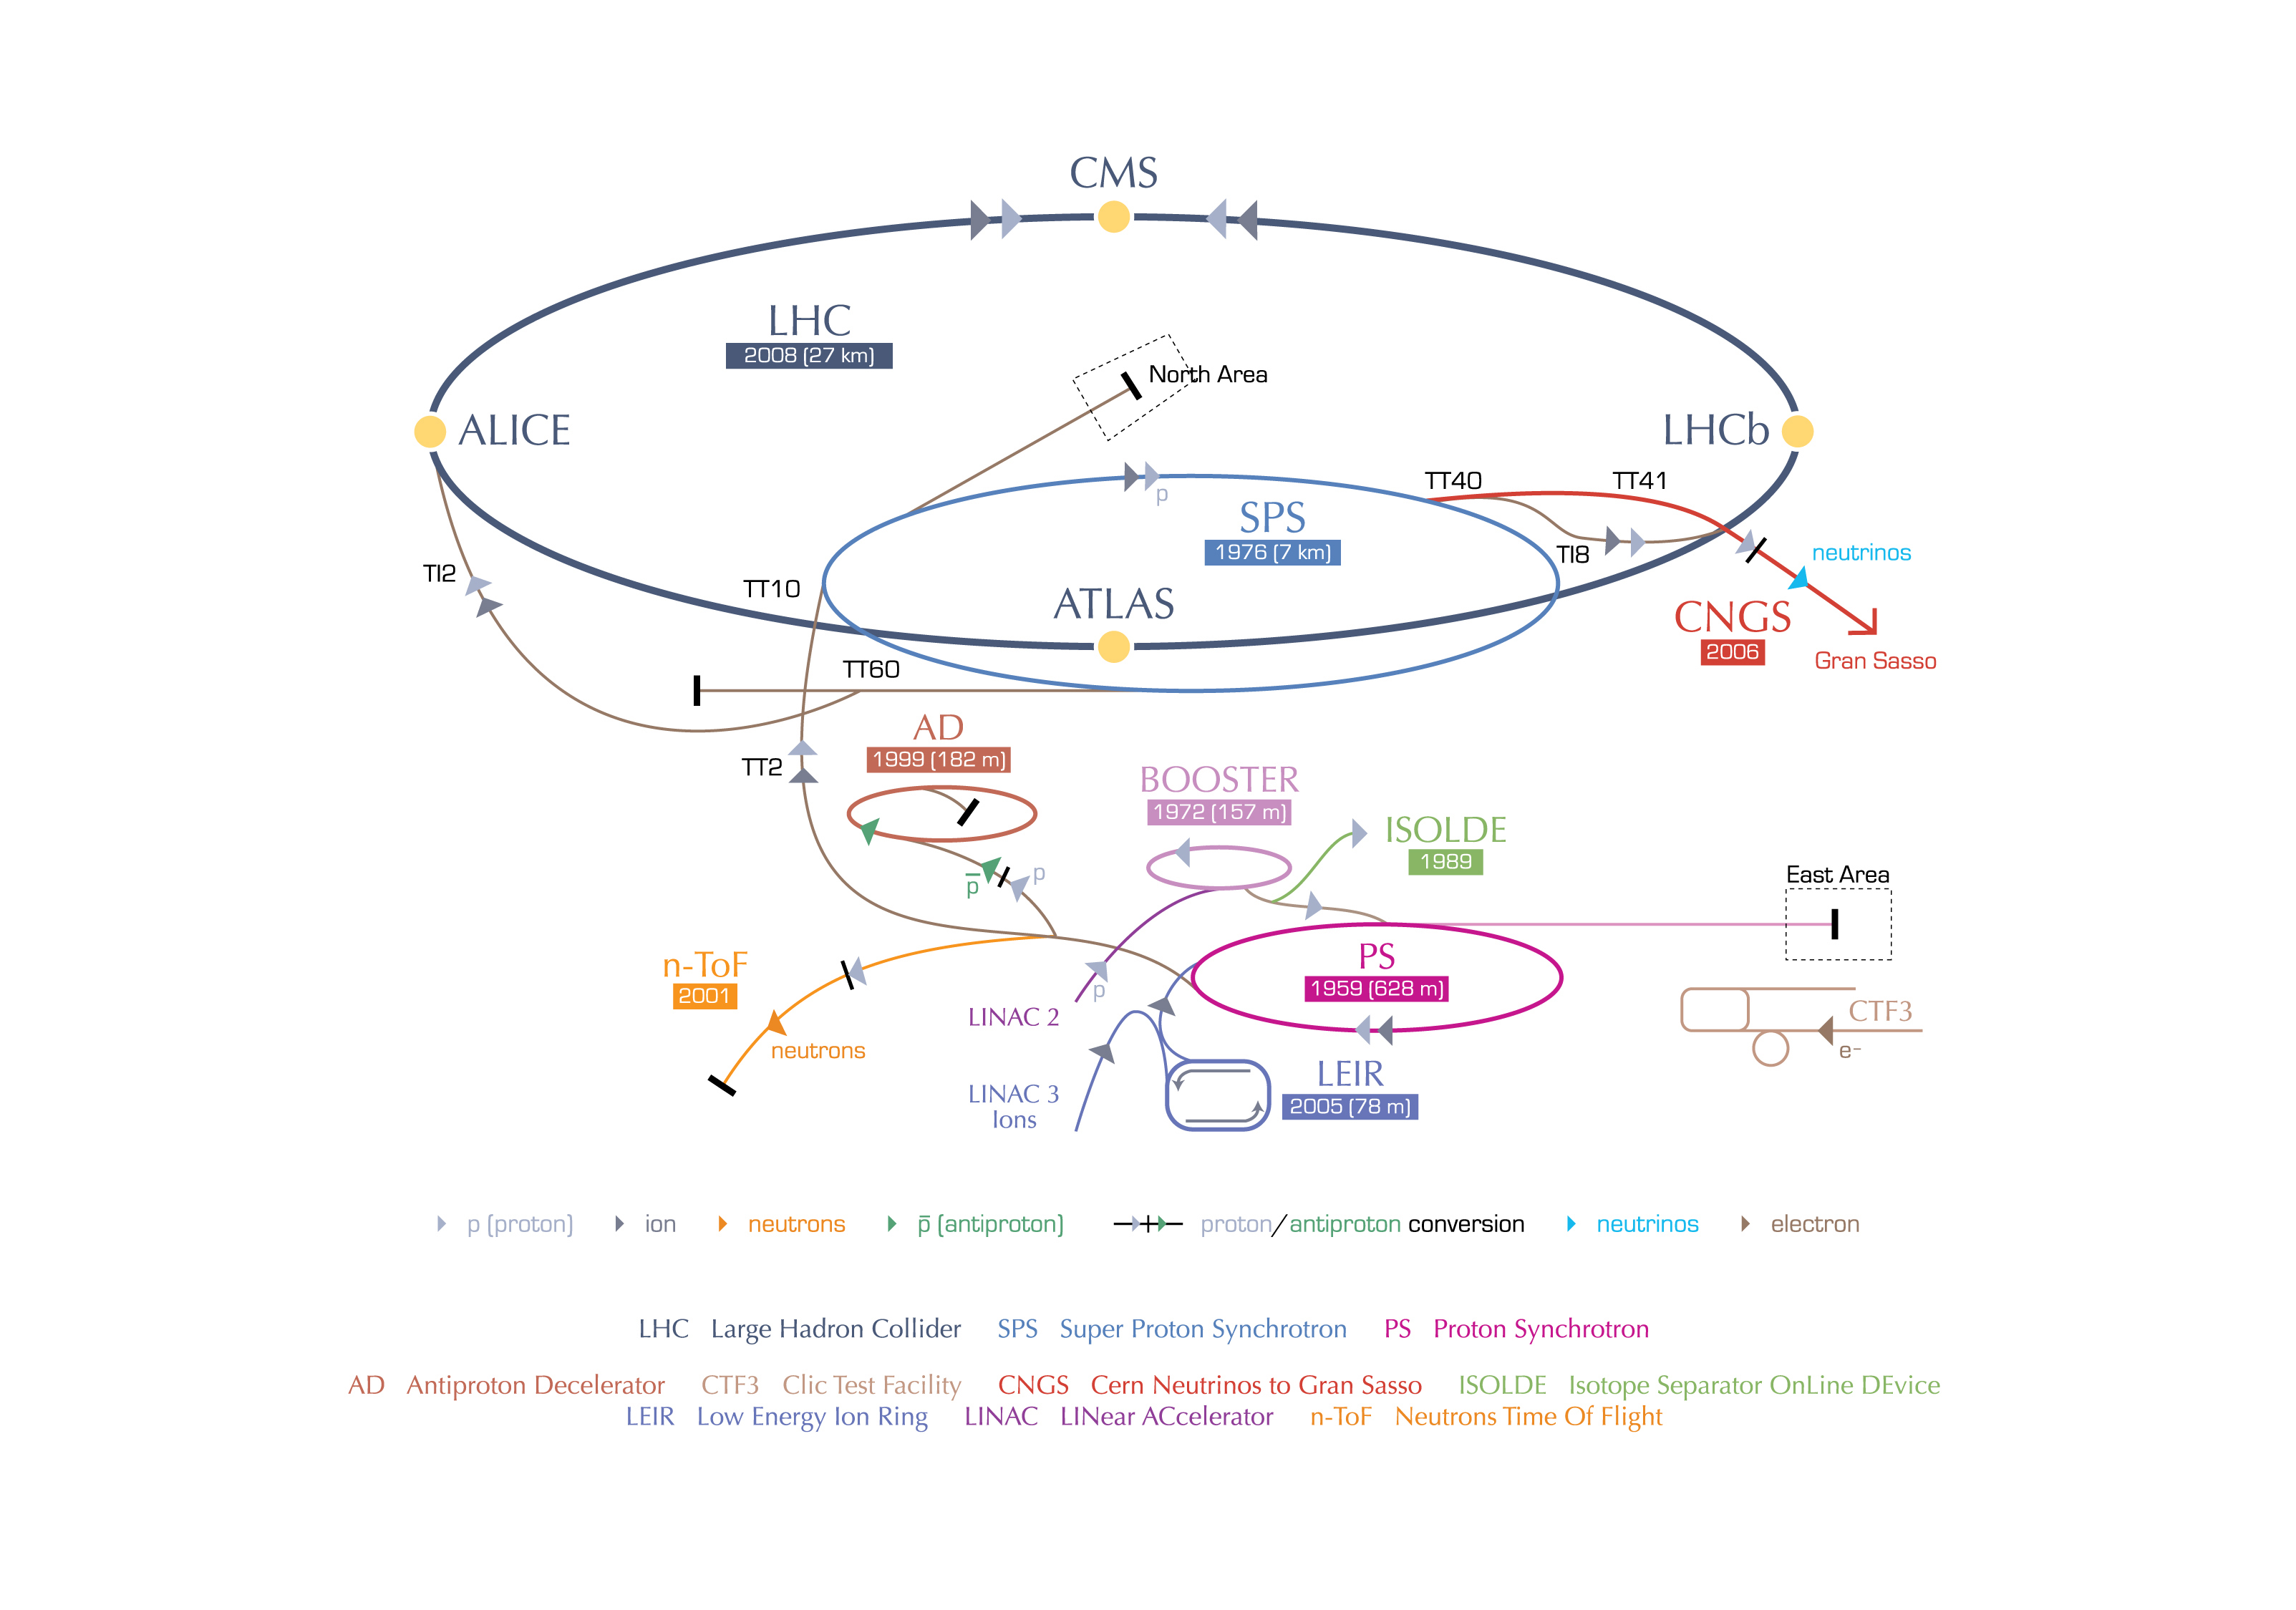
\includegraphics[width=1.0\textwidth]{figures/cms/LHC.jpg}
    \caption{The Large Hadron Collider accelerator complex. The four collision points along the ring correspond to the location of the LHC particle detectors CMS, LHCb, ATLAS and ALICE~\cite{LHC}.}
    \label{fig:cms:LHC}
\end{figure}

After the beams have reached their maximum energy and are stably circulating in the LHC ring, they are brought to collide. The goal of such a collision, which occurs every 25 nano seconds, is that some of the protons will undergo an inelastic collision, allowing the quark/gluon constituents of each proton to interact with one another and produce new and interesting particles.
The number of times such an interaction will take place inside a detector per area and time is quantified through the luminosity,$\mathcal L$, which is the proportionality factor between the number of observable events per second, and the cross section $\sigma$ of the process you are interested in
 
\begin{equation}
  \frac{dN_{events}}{dt} =\mathcal L \sigma .
\end{equation}

The cross section is the probability that an event (like one which would produce new and interesting particles) will occur and is measured in barns, where $1 \textrm{ barn} = 10^{-28} \textrm{ m}^2$. This proportionality factor should therefore be as high as possible. It depends only on parameters of the detector and can, in the case of LHC, be defined through the following accelerator quantities

\begin{equation}
  \mathcal L = \frac {N_b^2 n_b f_{rev} \gamma_r} {4 \pi \epsilon_n \beta *}F,
\end{equation}

where $N_b$ is the number of particles per bunch, $n_b$ is the number of bunches, $f_{rev}$ is their revolution frequency, $\gamma_r$ is the relativistic gamma factor,
$\epsilon_n$ is the transverse beam emittance (how confined the particles are in space and momentum), $\beta *$ is the beta function at the collision point (how narrow, or "squeezed", the beam is) and F is a reduction factor to account for a constellation where the beams do not collide heads-on but at slight crossing angles.
From this, it becomes clear that the main goal of the LHC is to; maximize the number of particles ($N_b$,$n_b$), their frequency ($f_rev$) and their energy ($\gamma_r$),
while at the same time ensuring the protons are packed together as tightly as possible (lower $\epsilon_n$ and $\beta *$).
Using the nominal values of the LHC, the peak luminosity is roughly $\mathcal L \sim 10^{34} \textrm{cm}^{-2} s^{-1}$. 


The peak luminosity of the LHC by the end of Run 2 in 2018 was grazing around $2.0 \cdot 10^{34} \textrm{cm}^{-2} s^{-1}$, corresponding to 2 times the nominal design luminosity.

To quantify the size and statistical power of a given LHC dataset, the integrated luminosity is used. This it the integral of the instantaneous luminosity over time and is defined as

\begin{equation}
  \mathcal L_{int} = \int \mathcal L dt.
\end{equation}

It is usually defined in units of inverse cross section, $\textrm{b}^{-1}$.


Despite the LHC starting up in 2008, there would be another year before data taking began.In March 2010, the LHC saw its first collision with a center-of-mass energy of 7 TeV, and continued running at this energy collecting around 5 inverse femtobarns of data by the end of 2011. In 2012, the energy was increased to 8 TeV and the LHC continued running until a planned long shutdown scheduled to begin in February 2013, collecting a total of $\sim 20 \textrm{ fb}^{-1}$ and discovering the Higgs boson. 
This marked the end of Run 1 and the beginning of a two-year maintenance project intended to prepare the LHC for running at a center-of-mass energy of 13 TeV; Run 2.

Run 2, and where this thesis begins, started in June 2015. With the accelerator now running at 90\% of its nominal energy, and with a peak luminosity between 1-2 times the design luminosity, the LHC managed to collect an impressive $\sim 160 \textrm{ fb}^{-1}$ at this energy until its planned shutdown at the end of 2018. Some key LHC accelerator parameters that were in use for the datasets analyzed in this thesis, are quoted in Table~\ref{tab:LHCparameters}

\begin{table}[]
\begin{tabular}{| l | lllll |}
\hline
Parameter               & Units                                   & Nominal & 2015 & 2016 & 2017     \\
\hline
Energy                  & {[}TeV{]}                               & 7.0     & 6.5  & 6.5  & 6.5      \\
Bunch spacing           & {[}ns{]}                                & 25      & 25   & 25   & 25       \\
Bunch intensity         & $\times10^{11}${[}protons/bunch{]}              & 1.15    & 1.15 & 1.15 & 1.2-1.45 \\
Bunches per train       &                                         & 144     & 144  & 96   & 144      \\
Total number of bunches &                                         & 2808    & 2244 & 2220 & 2556     \\
$\beta*$                & {[}cm{]}                                       & 55      & 80   & 40   & 27/25    \\
Peak luminosity         & $\times 10^{34} [\textrm{cm}^{-2} s^{-1}]$ & 1.0     & 0.5  & 1.4  & 2.0      \\
Integrated luminosity   &                                         &         & 4.2  & 39.7 & 50.2    \\
\hline
\end{tabular}
\caption{Some key LHC detector parameters achieved during the first years of 13 TeV data taking, 2015-2017.}
\label{tab:LHCparameters}
%https://indico.cern.ch/event/663598/contributions/2782540/,https://indico.cern.ch/event/580313/contributions/2359285/attachments/1396590/2135891/Operation_in_2016_v1_1.pdf, http://iopscience.iop.org/article/10.1088/1748-0221/3/08/S08001/pdf
\end{table}



 % with the full Run 2 (2016-2017) dataset corresponding to around$\sim 80\textrm{fb}^{-1}$.







\section{The CMS detector}
\subsection{Pixel detector and strip tracker}
\subsection{Electromagnetic calorimeter}
\subsection{Hadronic calorimeter}
\subsection{Muon chambers}
\section{Trigger system: From collision to disk}
